%%%%%%%%%%%%%%%%%%%%%%%%%%%%%%%%%%%%%%%%%%%%%%%%%%%%%%%%%%%%%%%
%
% Welcome to Overleaf --- just edit your LaTeX on the left,
% and we'll compile it for you on the right. If you open the
% 'Share' menu, you can invite other users to edit at the same
% time. See www.overleaf.com/learn for more info. Enjoy!
%
%%%%%%%%%%%%%%%%%%%%%%%%%%%%%%%%%%%%%%%%%%%%%%%%%%%%%%%%%%%%%%%


% Inbuilt themes in beamer
\documentclass{beamer}

% Theme choice:
\usetheme{CambridgeUS}

% Title page details: 
\title{Assignment 7} 
\author{Pradeep Mundlik (AI21BTECH11022)}
\date{\today}
% \logo{\large \LaTeX{}}


\begin{document}

% Title page frame
\begin{frame}
    \titlepage 
\end{frame}

% Remove logo from the next slides
% \logo{}


% Outline frame
\begin{frame}{Outline}
    \tableofcontents
\end{frame}

\section{Question}
\begin{frame}{Question}
    \begin{block}{Papoulis 3.8}
        A pair of dice is rolled n times. (a) Find the probability that "seven" will not show
at all. (b) (Pascal) Fmd the probability of obtaining double six at least once. 
    \end{block}
\end{frame}

\section{Answer}
\begin{frame}{Answer}
    The space of single roll of two dice consists of the 36 elements $f_if_j$, i, j = 1, 2, ..., 6. 
\end{frame}

\subsection{Part-1}
\begin{frame}{Part-1}
    Let A be the event \\
    A: Sum is seven \\
    The event A consist of six elements \\
    \begin{align}
        f_1f_6, f_2f_5, f_3f_4, f_4f_3, f_5f_2, f_6f_1 
    \end{align}
    Therefore, probability of A is
    \begin{align}
        P(A) = \frac{6}{36} = \frac{1}{6} \\
    \end{align}
    and 
    \begin{align}
        P(\bar{A}) &= 1 - P(A) \\
                   &= 1 - \frac{1}{6} = \frac{5}{6}
    \end{align}
\end{frame}

    \begin{frame}
        Therefore, for n trials 
        \begin{align}
            P_n(0) = \left(\frac{5}{6}\right)^n
        \end{align}
    \end{frame}
\begin{frame}
    \begin{figure}[!ht]
        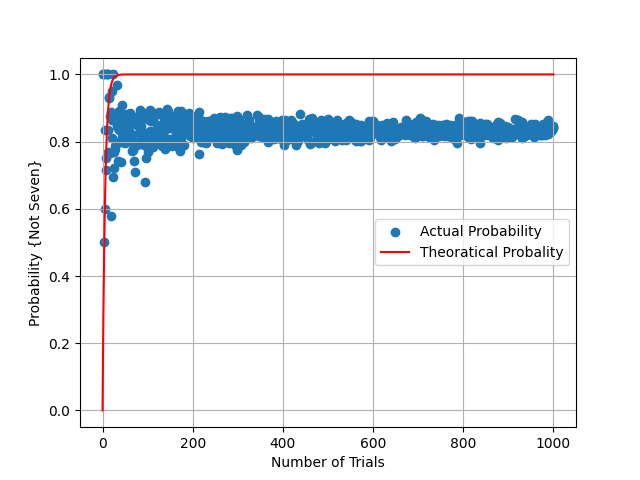
\includegraphics[width=4in, height=3in]{Figures/Figure_1.png}
    \end{figure}
\end{frame}
\subsection{Part-2}
\begin{frame}{Part-2}
    Let B be the event \\
    B: Double six \\
    The event B consist of only one element \\
    \begin{align}
        f_6f_6
    \end{align}
    Therefore, probability of B is
    \begin{align}
        P(B) = \frac{1}{36} \\
    \end{align}
    and probability of $\bar{B}$ is 
    \begin{align}
        P(\bar{B}) &= 1 - P(B) \\
        &= 1 - \frac{1}{36} = \frac{35}{36} \\
    \end{align}
\end{frame}
\begin{frame}
    Let \\
    $X$ = There will be atleast one double six in n rolls \\
    $\bar{X}$ = There will be no any double six in n rolls
    \begin{align}
        &\bar{X} = \bar{B}\times\bar{B}\times...\times\bar{B} \\
        \implies &P(\bar{X}) = \left(P(\bar{B})\right)^n \\
        \implies &P(\bar{X}) = \left(\frac{35}{36}\right)^n \\
        \implies &P(X) = 1 - P(\bar{X}) \\
        \implies &P(X) = 1 - \left(\frac{35}{36}\right)^n
    \end{align}
\end{frame}
\begin{frame}
    \begin{figure}[!ht]
        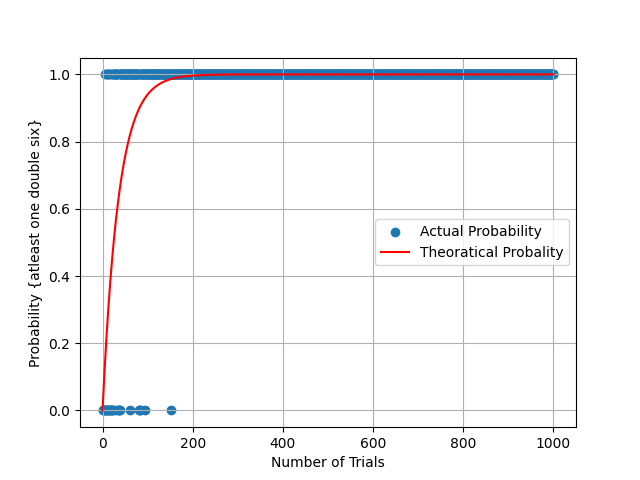
\includegraphics[width=4in, height=3in]{Figures/Figure_2.png}
    \end{figure}
\end{frame}
\end{document}